% !TeX document-id = {2d0db28c-3597-42a8-ab33-94df3552a9b8}
% This is samplepaper.tex, a sample chapter demonstrating the
% LLNCS macro package for Springer Computer Science proceedings;
% Version 2.21 of 2022/01/12
%
% !TeX spellcheck = en_US
% !BIB program = bibtex 
\documentclass[runningheads]{llncs}
%
\usepackage[T1]{fontenc}
% T1 fonts will be used to generate the final print and online PDFs,
% so please use T1 fonts in your manuscript whenever possible.
% Other font encondings may result in incorrect characters.
%
\usepackage{graphicx}
% Used for displaying a sample figure. If possible, figure files should
% be included in EPS format.
%
% If you use the hyperref package, please uncomment the following two lines
% to display URLs in blue roman font according to Springer's eBook style:
%\usepackage{color}
%\renewcommand\UrlFont{\color{blue}\rmfamily}
%\urlstyle{rm}
%

% Local packages
\usepackage{algorithm2e}
\usepackage{amssymb}
\usepackage[inline]{enumitem}
\usepackage{pifont}
\usepackage{subcaption}
\usepackage{tikz}
\usepackage{xcolor}
\usepackage{xfrac}

% tikz libraries
\usetikzlibrary{calc}
\usetikzlibrary{positioning}
\usetikzlibrary{bbox}

%%%% Local definitions %%%%
\newcommand{\bubblecoach}{\ensuremath{\texttt{P}_{\rm bubble}}\,}
\newcommand{\quickcoach}{\ensuremath{\texttt{P}_{\rm quick}}\,}
\newcommand{\learner}{learner}
\newcommand{\coach}{coach}
\newcommand{\NULL}{{\rm\texttt{null}}}
\newcommand{\learnerpolicy}{\texttt{P}_{\learner}}
\newcommand{\coachpolicy}{\texttt{P}_{\coach}}
\newcommand{\qmark}{\texttt{\textbf{?}}}
\newcommand{\ttus}{\char`_}

\newcommand{\searchpath}[2]{{search\_path(#1, #2)}}
\newcommand{\evaluate}[3]{{evaluate(#1, #2, #3)}}
\newcommand{\updatehypothesis}[1]{{update\_hypothesis(#1)}}

\newcommand{\partialadvice}[1]{partial@{#1}}

%%%% Color definitions
\definecolor{correctColor}{HTML}{19aa50}
\definecolor{wrongColor}{HTML}{aa1950}
\definecolor{adviceColor}{HTML}{1950aa}
\definecolor{unknownColor}{HTML}{ca8520}

\definecolor{bubbleColor}{HTML}{19aa50}
\definecolor{quickColor}{HTML}{aa1950}

%%%% algorithm2e macros
\SetKwRepeat{Do}{do}{while}
%%%%%%%%%%%%%%%%%%%%%%%%%%%

%%%% Editor's commands %%%%
\newcommand{\edcom}[1]{{\sf\color{red}$>>>$ #1}}
\newcommand{\tbc}{\edcom{To be completed\ldots}}
\setlength\marginparwidth{3cm}
\newcommand{\ednote}[1]{\marginpar{\flushleft\tiny\sf\color{red}{#1}}}
%%%%%%%%%%%%%%%%%%%%%%%%%%%

\begin{document}
%
\title{Title (Not ``Coaching How To Search'')}
%
%\titlerunning{Abbreviated paper title}
% If the paper title is too long for the running head, you can set
% an abbreviated paper title here
%
\author{Vassilis Markos\inst{1} \and
Loizos Michael\inst{1,2}}
%
\authorrunning{V. Markos, and L. Michael}
% First names are abbreviated in the running head.
% If there are more than two authors, 'et al.' is used.
%
\institute{Open University of Cyprus, Nicosia, Cyprus \and
CYENS Center of Excellence, Nicosia, Cyprus
\email{vasileios.markos@st.ouc.ac.cy,loizos@ouc.ac.cy}}
%
\maketitle              % typeset the header of the contribution
%
\begin{abstract}
The abstract should briefly summarize the contents of the paper in
150--250 words.

\keywords{First keyword  \and Second keyword \and Another keyword.}
\end{abstract}
%
%
%
\section{Introduction}\label{sec:Introduction}
%
\ednote{This should frame the work either as "implementations" of Machine Coaching --- statistical vs symbolic or so --- or as exploring problems which can be easily solved by (symbolic) Machine Coaching efficiently and providing full control over how the agent behaves vs formally not-guaranteed methods.}
%
%
%
\section{Related Literature}\label{sec:Related Literature}
%
\ednote{Reinforcement learning approaches might precede in this section.}
Several lines of work have examined how knowledge can pass between a machine learner and a human coach. One such line is eXplainable Interactive Learning (XIL) \cite{tesoKerstingIML2019}, in which a human supervisor acts as a learning ``coach'' and supplies advice that either corrects mislabeled data or revises incorrect explanations that the learner has offered for otherwise correct predictions. In Machine Coaching, by contrast, coach advice can be inserted directly into the learner's knowledge base in an elaboration-tolerant fashion \cite{mccarthyElaborationTolerance1998}, whereas XIL treats an active learning algorithm as a black-box \cite{Settles2009ActiveLL} together with a local post-hoc explainer \cite{ribeiro2016}. The resulting explanations are then used to produce further labeled data that help the learner resolve misunderstandings.

User feedback can likewise be employed to reduce, in advance, the amount of data-point labeling that is required, as illustrated for Support Vector Machines in \cite{raghavanAllan2007}. Along related lines, \cite{settles-2011-closing} introduces an interactive setting in which users label selected data points so as to refine the training of a document classifier, while \cite{zaidan2007using} puts forward a machine learning approach that relies on user-provided explanations to lower learning complexity. Notably, \cite{zaidan2007using} emphasizes that, as an alternative to relying on large volumes of data for better performance, one may seek \emph{data richness}, that is, more informative data such as a correct label accompanied by an explanation. \emph{Coactive Learning}, introduced in \cite{shivaswamyJoachims2015}, is a further interactive Machine Learning framework in which the learner obtains user advice that is, by design, only ``slightly better'' than the learner's current prediction. As shown in \cite{shivaswamyJoachims2015}, a principal advantage of this approach is that it can be incorporated into many existing black-box methodologies.

Beyond supporting faithfulness and fostering user trust \cite{BARREDOARRIETA202082}, embedding explanations during model training has been found to raise testing performance \cite{Selvaraju_2019}. In addition, bilateral explanations---from the learner to the coach and from the coach to the learner---can accelerate learning still further \cite{dongSu2017}, and comparable gains arise when models are retrained with extra explanations for decisions that are wrong, or that are correct but for the wrong reasons \cite{riegerSingh2019}. Finally, post-hoc fine tuning of models also yields performance gains \cite{ribeiro2016}.

In light of the recent surge in the use of Large Language Models (LLMs) across nearly every domain, methods for human--machine interaction that leverage human expertise to refine an LLM have been put forward. \cite{welz2024} presents a human knowledge infusion approach in which expert users contribute domain-specific knowledge that populates a knowledge base, which the system then combines with the LLM when answering user queries. Analogously, \cite{wang2024} describes a human--LLM collaborative data annotation scheme in which the human supervises the LLM by revising and correcting erroneous data labels and/or the associated LLM explanations, in the spirit of \cite{tesoKerstingIML2019}. In \cite{kim2024megannohumanllmcollaborativeannotation}, human--LLM collaboration is studied in a setting where the user may freely explore, correct, and interact with LLM responses via suitable programmatic interfaces or interface widgets. A related variant, in which human supervisors freely inspect and correct LLM annotations in PDF files, is proposed in \cite{tang2024}. In robotics, human robot teleoperators have been assigned coaching roles in hybrid robot--LLM systems so as to verify system decisions \cite{liu2023llmbasedhumanrobotcollaborationframework}. For generative design customization, passive, assistive, and proactive human--LLM collaboration schemes have been suggested \cite{WANG2025425}, each geared toward users with different levels of expertise.

It is worth recalling that knowledge exchange between a coach and a machine learner---in the form of context-driven advice predicated on the learner's decisions---was already described in \cite{mccarthyProgramsCommonSense1959}. More recently, it has been formalized under the heading of \emph{Machine Coaching} \cite{michaelAdviceTaker2017,michaelMachineCoaching2019} within the Probably Approximately Correct (PAC) model \cite{valiantPAC1984}.

Although AI system verification and faithful embedding of human expertise have received substantial attention, the focus is typically on what the machine learner can ultimately achieve and how successful it is. Yet there are many applications in which this desideratum is secondary to \emph{``how''} the machine learner attains its goals. Deep neural architectures and LLMs, despite their prevalence in most applications owing to their efficiency and efficacy, are not necessarily the most suitable vehicles for exact human knowledge representation, partly because they lack solid formal guarantees on their behavior. Argumentation-based approaches \cite{DUNG1995321,prakkenAnAbstractFrameworkFA2010}, by contrast, come with such guarantees ``out-of-the-box'', and may therefore serve as a useful instrument in the design of cognitive agents in such settings.
%
%
%
\section{Learning Faithful Sorting Using RL}\label{sec:Learning Faithful Sorting using RL}
%

%
%
%
\section{Learning Faithful Sorting Using Symbolic Policies}
%

%
%
%
\subsection{Background and Preliminaries}\label{sec:background and preliminaries}
%
Building on the learning semantics introduced in earlier work on Machine Coaching \cite{michaelMachineCoaching2019,prudens2022}, we empirically investigate their application to search coaching. A machine learner repeatedly requests advice from a machine coach that emulates a human coach, as in \cite{proxyCoaching2022}, with the goal of progressively strengthening its search capacity under the coach's explicit search policy. Given a fixed goal state, $g$, the learner applies its search policy, $\learnerpolicy$, to find a path, $p$, that begins at an arbitrary state, $s$, and terminates at a goal state, $g$. Whenever knowledge is lacking, the learner asks its coach for advice; the coach replies according to its own policy, $\coachpolicy$, by returning a single piece of advice. Each piece of advice takes the form of an ``if-then'' rule whose \emph{body} (the ``if'' part) depends on the state and whose \emph{head} (the ``then'' part) is always an action to be taken by the learner. As in prior work \cite{proxyCoaching2022,prudens2022,ioannouKnowledgeBasedTranslationNatural2021}, the coach assigns priorities to rules so that, by default, later advice overrides earlier advice in $\learnerpolicy$, unless the coach specifies otherwise. In this setting, a \emph{coaching step} consists of one learner request for advice together with the matching coach response, whereas a \emph{coaching session} spans the entire learning cycle and ends once the learner has constructed a path as required (cf.\ Algorithm~\ref{alg:coaching process}). In every case, the learner requests advice when it lacks knowledge for continuing the search, and returns a partial path $p$ starting from $s$.

\begin{figure}[!tb]
	\centering
	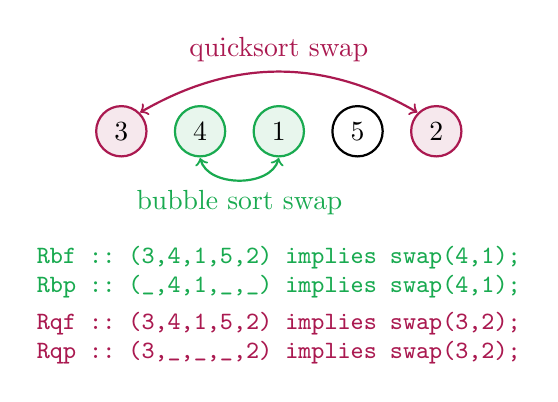
\begin{tikzpicture}[
		bezier bounding box,
		arrow/.style={->, draw=black, thick},
		advice/.style={draw=adviceColor, densely dotted},
		node/.style={circle, inner sep=0.125cm, outer sep=0.2mm, draw=black, thick},
		faded/.style={opacity=0.2},
		bubble/.style={draw=bubbleColor, fill=bubbleColor, fill opacity=0.1, text opacity=1.0},
		quick/.style={draw=quickColor, fill=quickColor, fill opacity=0.1, text opacity=1.0},
		unknown/.style={draw=unknownColor, fill=unknownColor, fill opacity=0.1},
		text box/.style={font=\tt},
	]
	% State nodes
	\node[node, quick] (state 1) at (1, 0) {3};
	\node[node, bubble] (state 2) at (2, 0) {4};
	\node[node, bubble] (state 3) at (3, 0) {1};
	\node[node] (state 4) at (4, 0) {5};
	\node[node, quick] (state 5) at (5, 0) {2};
	% Rules
	\node[text box, below={of state 3.south}, anchor=north, bubbleColor] (full bubble) {\bfseries\small Rbf ::~(3,4,1,5,2) implies swap(4,1);};
	\node[text box, below={0.1cm of full bubble.south west}, anchor=west, bubbleColor] (partial bubble) {\bfseries\small Rbp ::~(\ttus,4,1,\ttus,\ttus) implies swap(4,1);};
	\node[text box, below={0.2cm of partial bubble.south west}, anchor=west, quickColor] (full quick) {\bfseries\small Rqf ::~(3,4,1,5,2) implies swap(3,2);};
	\node[text box, below={0.1cm of full quick.south west}, anchor=west, quickColor] (partial quick) {\bfseries\small Rqp ::~(3,\ttus,\ttus,\ttus,2) implies swap(3,2);};
	% Swap arrows
	\draw[<->, thick, bubbleColor] (state 2.south) to[bend right, in=255, out=-75] node[pos=0.5, below]{bubble sort swap} (state 3.south);
	\draw[<->, thick, quickColor] (state 1.north east) to[bend left] node[pos=0.5, above]{quicksort swap} (state 5.north west);
\end{tikzpicture}
	\caption{Examples of full (\texttt{f}) and partial (\texttt{p}) advice from \bubblecoach (\texttt{b}) and \quickcoach (\texttt{q}) on state $(3,4,1,5,2)$.}
	\label{fig:sorting rules}
\end{figure}


\begin{algorithm}
	\caption{Search coaching process. $s$, $g$ denote the start and goal states, respectively.}%
	\label{alg:coaching process}
	\KwData{$s$, $g$, $\learner$, $\coach$}
	\KwResult{$\learner$ with updated search policy; $path$ from $s$ to $g$.}
	%	$advice\gets\NULL$\;
	\Do{advice is not \NULL}{%
		$path \gets \learner.\searchpath{s}{g}$\;
		$advice \gets \coach.\evaluate{path}{s}{g}$\;
		$\learner.\updatehypothesis{advice}$\;
	}
\end{algorithm}

We consider the special case of sorting cast as a search problem, and implement two coaching \emph{policies}: \bubblecoach, grounded in bubble sort, and \quickcoach, grounded in quicksort. In both cases, advice corresponds to the next step of the algorithm embodied by the coaching policy. A state of size $n$ is any permutation of $\{1,2,\ldots,n\}$; start states are chosen arbitrarily among all states of that size, while the goal state is invariably $(1,2,\ldots,n)$. Rules then take as their body a potentially partial permutation of $\{1,2,\ldots,n\}$ and as their head a swap of two items in that permutation, as illustrated in Figure~\ref{fig:sorting rules}.

\begin{figure}[!tb]
	\centering
	\begin{tikzpicture}[
		bezier bounding box,
		arrow/.style={->, draw=black, thick},
		advice/.style={draw=adviceColor, densely dotted},
		node/.style={circle, inner sep=0.125cm, outer sep=0.2mm, draw=black, thick},
		faded/.style={opacity=0.2},
		correct/.style={draw=correctColor, fill=correctColor, fill opacity=0.1, label={center, text=correctColor}:{\small\checkmark}},
		wrong/.style={draw=wrongColor, fill=wrongColor, fill opacity=0.1, label={center, text=wrongColor}:{\small\ding{55}}},
		unknown/.style={draw=unknownColor, fill=unknownColor, fill opacity=0.1, label={center, text=unknownColor}:{\qmark}},
		text box/.style n args={1}{text width={#1cm}}
	]
	% Nodes
	\foreach \i/\j/\lab in {0/0/a, 2/2/b, 0.3/0.7/c} {
		\node[node, faded] (\lab) at (\i, \j) {};
	}
	\foreach \i/\j/\lab in {1/2/d, 2.5/0/e} {
		\node[node, correct] (\lab) at (\i, \j) {};
	}
	\foreach \i/\j/\lab in {1.4/1/g, 3/1/h} {
		\node[node, wrong] (\lab) at (\i, \j) {};
	}
	\node[node, unknown] (f) at (1.3, 0.1) {};

	% Arrows
	\foreach \s/\goal in {d/g, e/f} {
		\draw[arrow, correctColor] (\s) -- (\goal);
	}
	\foreach \s/\goal in {g/h, h/e} {
		\draw[arrow, wrongColor] (\s) -- (\goal);
	}
	\foreach \s/\goal in {g/c, h/f, f/a} {
		\draw[arrow, advice] (\s) -- (\goal);
	}
	\foreach \s/\goal in {d/c, d/b, g/b, c/f, b/h} {
		\draw[arrow, faded] (\s) -- (\goal);
	}

	% Text boxes
	\node[text box={1.4}] (proactive) at (-0.8,2.2) {Proactive Coaching};
	\node[text box={1.4}] (reactive) at (-0.8,-0.9) {Reactive Coaching};
	\node[text box={1.4}] (reflexive) at (4.2,2.2) {Reflexive Coaching};
	
	% Text box to graph arrows
	\draw[arrow, thin, dashed] ($(g)!0.5!(c)$) to[bend right] (proactive);
	\draw[arrow, thin, dashed] ($(f)!0.5!(a)$) to[bend left] (reactive);
	\draw[arrow, thin, dashed] ($(f)!0.5!(h)$) to[bend left] (reflexive);
	
	% Legend
	\node[anchor=north west, draw=black!40, rounded corners=0.2cm, inner sep=0.1cm] (legend) at (2.6,-0.3) {%
		\begin{tikzpicture}
			\pgfmathsetmacro{\dx}{0.4}
			\pgfmathsetmacro{\dy}{0.4}
			\draw[ultra thick, correctColor] (0,0) -- (\dx,0) node[pos=1, right] {correct action};
			\draw[ultra thick, wrongColor] (0,-\dy) -- (\dx,-\dy) node[pos=1, right] {wrong action};
			\draw[ultra thick, adviceColor, densely dotted] (0,{-2*\dy}) -- (\dx,{-2*\dy}) node[pos=1, right] {advised action};
		\end{tikzpicture}%
	};
\end{tikzpicture}
	\caption{Different coaching styles used in the experimental setup. Upon the learner reaching a state from where there is no knowledge on how to proceed (\textcolor{unknownColor}{\qmark}), a reactive piece of advice resolves this lack of knowledge, a proactive piece of advice addresses the first wrong decision in the learner's search path, while a reflexive piece of advice addresses a random mistake / lack of knowledge of the learner.}
	\label{fig:coaching styles}
\end{figure}

Within this setting, two advice types are distinguished:
\begin{enumerate*}[label=(A\arabic*)]
	\item \emph{full advice}, in which each piece of advice depends on the entire state, and;
	\item \emph{partial advice}, in which each piece of advice depends on the particular portion of the state that is to be improved.
\end{enumerate*}
Furthermore, for each advice type three learner configurations concerning advice memorization have been examined:
\begin{enumerate*}[label=(M\arabic*)]
	\item \emph{no memory} across distinct iterations for a fixed state size, $n$, so that coaching sessions and the associated learned policies are pairwise independent;
	\item \emph{short memory} across distinct iterations for a fixed state size, $n$, so that coaching sessions for different values of $n$ are independent, whereas those for the same value of $n$ are not, and;
	\item \emph{long memory} across all values of state size, $n$, so that every coaching session is correlated and knowledge is built incrementally from all preceding test cases.
\end{enumerate*}
A coach may follow one of the \emph{coaching styles} depicted in Figure~\ref{fig:coaching styles}:
\begin{enumerate*}[label=(C\arabic*)]
	\item \emph{reactive} coaching, in which the coach advises on the learner's last wrong decision in $p$;
	\item \emph{reflexive} coaching, in which the coach advises on a randomly chosen wrong decision in $p$, and;
	\item \emph{proactive} coaching, in which the coach advises on the learner's earliest wrong decision in $p$.
\end{enumerate*}

\begin{figure*}[!tb]
	\centering%
	\hfill%
	\begin{subfigure}[t]{0.33\textwidth}
		\centering
		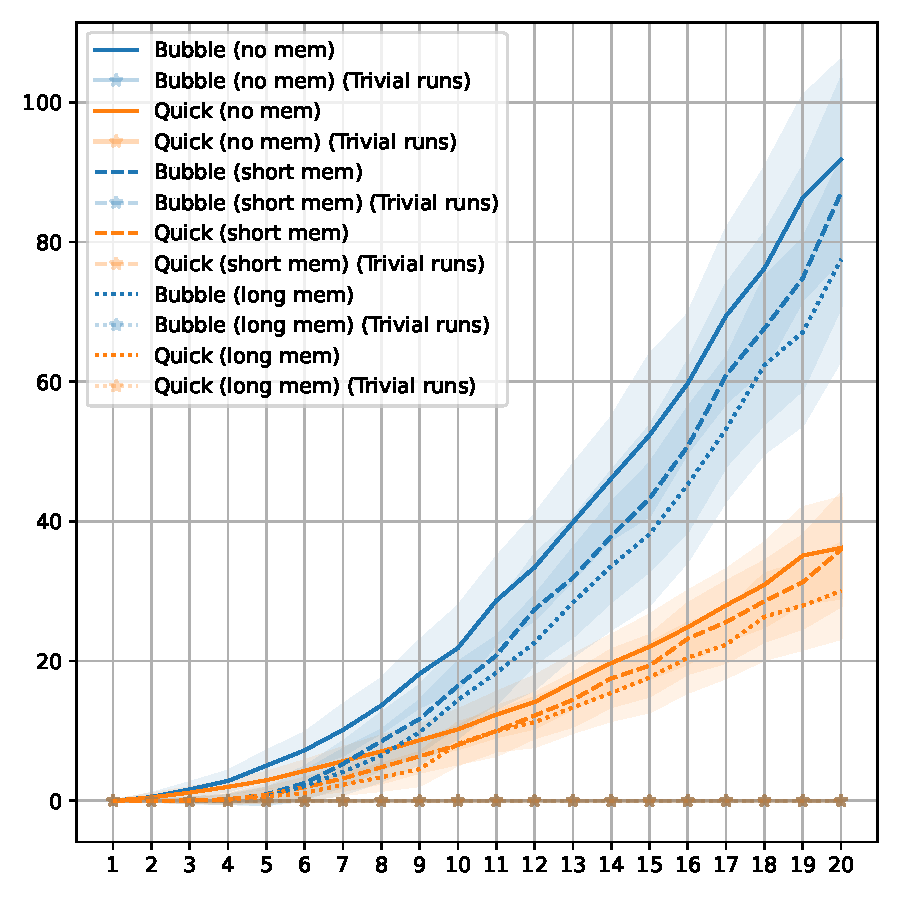
\includegraphics[width=\linewidth]{assets/images/a_20_100_full.pdf}
		\caption{Full advice, reactive coaching}
		\label{fig:full sorting coaching results a}
	\end{subfigure}%
	\hfill%
	\begin{subfigure}[t]{0.33\textwidth}
		\centering
		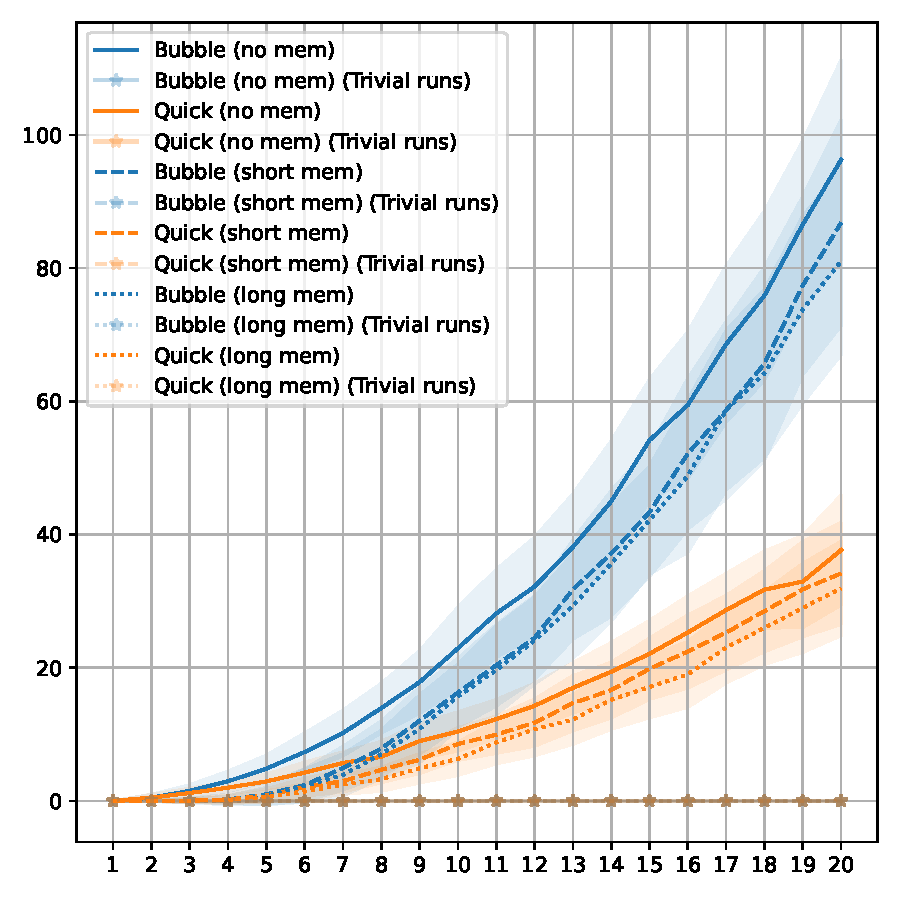
\includegraphics[width=\linewidth]{assets/images/r_20_100_full.pdf}
		\caption{Full advice, reflexive coaching}
		\label{fig:full sorting coaching results r}
	\end{subfigure}%
	\hfill%
	\begin{subfigure}[t]{0.33\textwidth}
		\centering
		
\includegraphics[width=\linewidth]{assets/images/p_20_100_full.pdf}
		\caption{Full advice, proactive coaching}
		\label{fig:full sorting coaching results p}
	\end{subfigure}%
	\hfill\\[1em]%
	\hfill%
	\begin{subfigure}[t]{0.33\textwidth}
		\centering
		
\includegraphics[width=\linewidth]{assets/images/a_20_100_partial.pdf}
		\caption{Partial advice, reactive coaching}
		\label{fig:partial sorting coaching results a}
	\end{subfigure}%
	\hfill%
	\begin{subfigure}[t]{0.33\textwidth}
		\centering
		
\includegraphics[width=\linewidth]{assets/images/r_20_100_partial.pdf}
		\caption{Partial advice, reflexive coaching}
		\label{fig:partial sorting coaching results r}
	\end{subfigure}%
	\hfill%
	\begin{subfigure}[t]{0.33\textwidth}
		\centering
		
\includegraphics[width=\linewidth]{assets/images/p_20_100_partial.pdf}
		\caption{Partial advice, proactive coaching}
		\label{fig:partial sorting coaching results p}
	\end{subfigure}%
	\hfill\\[1em]%
	\caption{Coaching steps as a function of state size, $n$. Full and partial advice (top and bottom, respectively) with reactive, reflexive and proactive coaching styles are considered (left, middle, and right, respectively), with all possible coach (\bubblecoach, \quickcoach) and memory (none, short, long) combinations are shown.}
	\label{fig:full and partial sorting coaching results}
\end{figure*}
%
%
%
\subsection{Experimental Setup}\label{sec:experimental setup}
%
We ran a series of experiments first to verify learning efficacy, where we let state size, $n$, range from $1$ to $20$, running $m=100$ iterations for each value of $n$. We have consider all possible combinations of advice type (full and partial), memory configurations (none, short, long), coaching styles (reactive, reflexive, proactive), and coaching policies (\bubblecoach and \quickcoach), resulting into 36 different coaching settings.

In order to explore how much the learner conforms to the coach's instructions in the various settings explored, we define \emph{coaching conformity} to be the relative frequency of learner decisions conforming to coach decisions on the same states over all such decisions in a session. First, we sample $m=20$ repetitions for state size $n\in\{5,10,15,20\}$ and compute coaching conformity for each one, across all coach policies, coaching styles, and memory configurations. Then, aiming to shed more light on the parameters affecting coaching conformity, we introduce a new type of advice, \partialadvice{k}, $2\leq k\leq n$, where $k-2$ randomly selected state variables are included into the advice condition, alongside the two required to describe the swap action of interest. Such advice captures intermediate levels of specificity between the two extremes explored so far, with \partialadvice{2} corresponding to partial and \partialadvice{n} to full advice for state size $n$. We also define \emph{advice coverage} as the percentage of state variables that is included in the condition of a piece of advice. So, e.g., a rule like \texttt{R ::~(\ttus,2,1,\ttus,5) implies swap(2,5)} has an advice coverage of $\sfrac{3}{5}=60\%$. Again, we ran $m=20$ iterations for state size $n\in\{5,10,15,20\}$, $2\leq k\leq n$, for all coaching policies, coaching styles, and memory configurations.

\subsection{Results}\label{subsec:sorting-results}
%
Figure~\ref{fig:full and partial sorting coaching results} reports, for each of the three coaching styles, the number of coaching steps needed to reach the goal state as a function of state size, $n$. In every setting except partial advice with reflexive coaching, the learner successfully finished all coaching sessions with the intended outcomes. For reactive coaching with full advice (Fig.~\ref{fig:full sorting coaching results a}), employing either short or long memory does not seem to alter the number of coaching steps in any notable way, as anticipated given the limited applicability of the advice that is supplied. By contrast, partial advice (Fig.~\ref{fig:partial sorting coaching results a}) together with short or long memory yields fewer coaching steps, which can be explained symmetrically by the wider applicability of that advice. Observe also that, under full advice, the number of coaching steps scales in proportion to the big-O complexity of the underlying policy / sorting algorithm---again a consequence of restricted advice applicability, which effectively obliges the learner to request step-by-step guidance in each distinct case. Juxtaposed with the full-advice setting, the use of memory markedly cuts the coaching steps required per session, because the learner can then reuse previously acquired knowledge on new cases. Note further that, under long memory (Fig.~\ref{fig:partial sorting coaching results a}), the coaching-step curves for \bubblecoach and \quickcoach essentially coincide (dotted lines), suggesting that, with reactive coaching, retaining all prior advice eventually lets the learner generalize and reach the goal state largely without frequent interaction with its ``lazy'' supervisor.

Turning to proactive coaching, where advice targets the learner's first wrong decision (Figs.~\ref{fig:full sorting coaching results p}, \ref{fig:partial sorting coaching results p}), full advice induces the same growth patterns in coaching steps as under reactive coaching. Supplying partial advice, however, substantially lowers the number of coaching steps per session---as with reactive coaching---since memory enables the learner to generalize from earlier cases. Notably, coaching steps remain systematically higher than in the corresponding reactive-coaching settings (Figs.~\ref{fig:partial sorting coaching results a}, \ref{fig:partial sorting coaching results p}). This mirrors the more ``meticulous'' interaction pattern of a proactive coach, which issues (even partial) advice that is more accurate and thereby curtails unnecessary exploration of the search space, at the expense of more frequent interaction with the learner than a reactive coach, which merely responds when further knowledge is requested.

For reflexive coaching (Figs.~\ref{fig:full sorting coaching results r}, \ref{fig:partial sorting coaching results r}), the trends mirror those of proactive coaching. Here, however, the coach's random choice of intervention state raises the possibility that the same piece of advice is issued more than once. Sessions of this kind are counted as \emph{trivial runs}. As state size increases, so does the number of trivial runs, particularly under non-trivial memory configurations, where the learner's policy tends to be larger and it is therefore generally more likely that the same advice is received repeatedly.

Finally, observe that the coaching policy ceases to matter once the learner has some form of memory, irrespective of advice type. For full advice this is expected, given that limited advice applicability prevents reuse of prior knowledge; partial advice, by contrast, lets the learner generalize in accordance with $\coachpolicy$ and thereby reduces the need for coach feedback. Focusing on partial advice without memory, reactive coaching produces sessions whose length scales with the complexity of the coaching policy, as noted above. The same does not hold for proactive and reflexive coaching, where the coach interacts with the learner more often---suggesting that, under reactive coaching, the learner may acquire an efficacious yet unfaithful policy, a phenomenon less likely under the other coaching styles.

\begin{figure*}
	\centering\hfill%
	
\includegraphics[width=0.33\textwidth]{assets/images/fidelity_test_N20_reps20_step5_coach_a.pdf}\hfill%
	
\includegraphics[width=0.33\textwidth]{assets/images/fidelity_test_N20_reps20_step5_coach_r.pdf}\hfill%
	
\includegraphics[width=0.33\textwidth]{assets/images/fidelity_test_N20_reps20_step5_coach_p.pdf}\hfill%
	\caption{Coaching fidelity against state size for reactive (left), reflexive (middle) and proactive (right) coaching.}
	\label{fig:coaching fidelities}
\end{figure*}

Figure~\ref{fig:coaching fidelities} plots average coaching conformity against state size, $n$. Irrespective of memory configuration, full advice paired with reactive coaching yields a virtually fully conformant learner that replicates the coach's policy. Comparable outcomes arise for proactive and reflexive coaches as well. With partial advice, however, coaching conformity hinges on coaching style and memory configuration. In particular, under reactive coaching, partial advice drives conformity to near zero for every memory configuration. Under proactive coaching, by contrast, partial advice sustains consistently high conformity across all examined state sizes, with little sensitivity to memory configuration. Reflexive coaching likewise produces higher conformity than reactive coaching, broadly echoing the proactive results. Observe also that coach type does not influence conformity in any setting except partial advice with reactive coaching, where apparent differences diminish as state size grows.
%
\begin{figure*}
	\centering\hfill%
	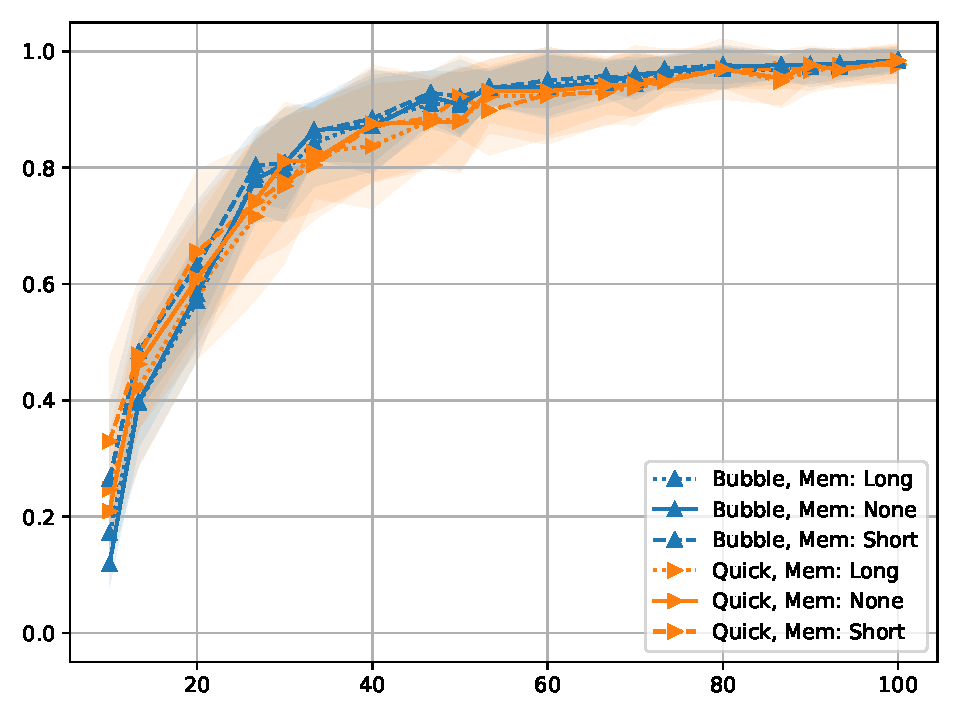
\includegraphics[width=0.33\textwidth]{assets/images/pper_fidelity_test_N20_reps20_step5_coaches3_partial_2_20_coach_a.pdf}\hfill%
	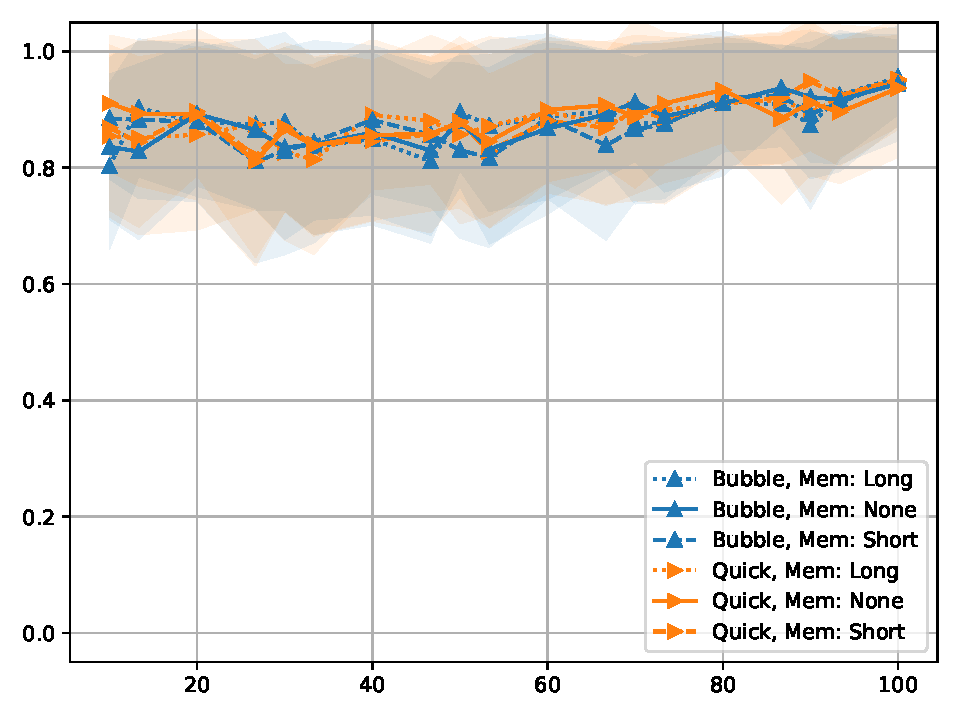
\includegraphics[width=0.33\textwidth]{assets/images/pper_fidelity_test_N20_reps20_step5_coaches3_partial_2_20_coach_r.pdf}\hfill%
	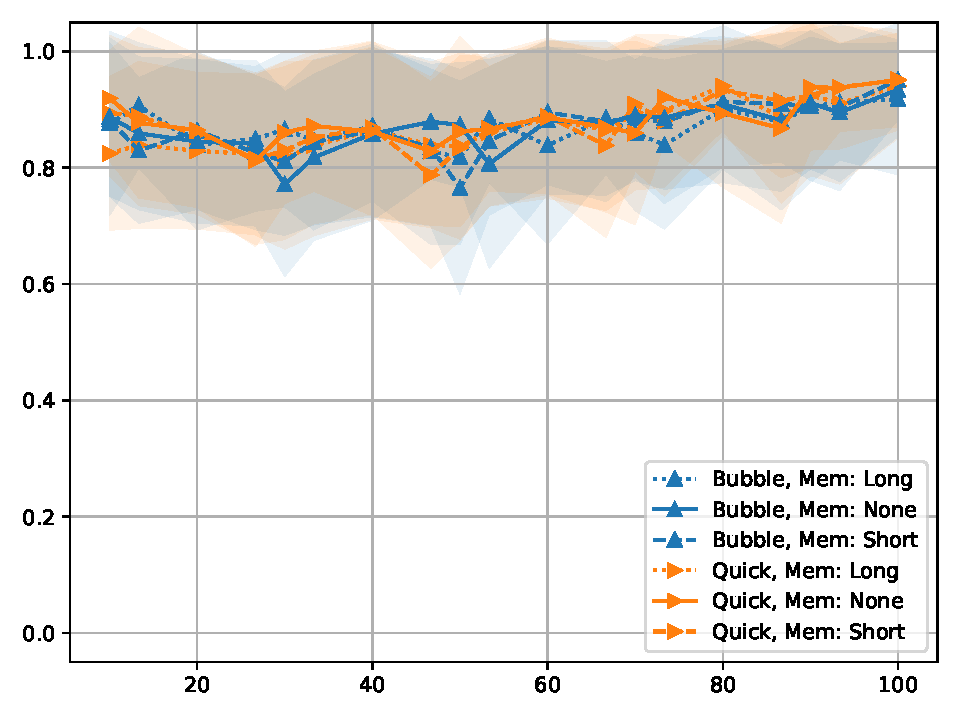
\includegraphics[width=0.33\textwidth]{assets/images/pper_fidelity_test_N20_reps20_step5_coaches3_partial_2_20_coach_p.pdf}\hfill%
	\caption{Coaching fidelity against advice coverage for reactive (left), reflexive (middle) and proactive (right) coaching.}
	\label{fig:fidelities against coverage}
\end{figure*}
%
Taken together, Figure~\ref{fig:coaching fidelities} points to a trade-off between advice specificity and coaching conformity: more specific advice yields greater conformity to the coaching policy, whereas looser advice affords more room for the learner to generalize from prior knowledge.

Figure~\ref{fig:fidelities against coverage} presents coaching conformity against advice coverage for all coaching policies and styles, aggregated over state size, $n$. Coaching policy and memory configuration leave conformity largely unaffected; the dominant factor is coaching style. Under reactive coaching, low advice coverage lets the learner reach the goal state without conforming to the coach's search policy, whereas more specific advice makes the learner's search steps toward the goal more accurate. Under proactive and reflexive coaching, by contrast, conformity rises only slightly with advice coverage and remains relatively high even at lower coverage values. Relative to reactive coaching, proactive and reflexive coaching appear to sustain a stably high conformity and to mitigate the drawbacks of arbitrarily low coverage almost equally well. In effect, earlier coach intervention keeps the learner from straying far from the coach's guidance, even when advice is minimal and leaves room for generalization.
%
%
%
\section{Conclusions}\label{sec:Conslusions}
%
%
%
\bibliographystyle{splncs04}
\bibliography{references}


\end{document}
